\chapter{Underwater granular flows}

\ifpdf
    \graphicspath{{Chapter6/figs/raster/}{Chapter6/figs/pdf/}{Chapter6/figs/}}
\else
    \graphicspath{{Chapter6/figs/vector/}{Chapter6/figs/}}
\fi

\section{Submarine granular flows down incline plane}

The flow of dense granular material is a common phenomenon in engineering predictions, such as avalanches, landslides, and debris-flow modelling. Despite the huge amount of research that has gone into describing the behaviour of granular flows, a constitutive equation that describes the overall behaviour of a flowing granular material is still lacking. The initiation and propagation of submarine granular flows depend mainly on the slope, density, and quantity of the material destabilised. Although certain macroscopic models are able to capture the simple mechanical behaviours, the complex physical mechanisms that occur at the grain scale, such as thydrodynamic instabilities, the formation of clusters, collapse, and transport, have largely been ignored~\citep{Topin2011}. The momentum transfer between the discrete and the continuous phases significantly affects the dynamics of the flow~\citep{Peker2007}. Grain-scale description of the granular material enriches the macro-scale variables,  which poorly account for the local rheology of the materials.  In order to describe the mechanism of saturated and/or immersed granular flows, it is important to consider both the dynamics of the solid phase and the role of the ambient fluid~\citep{Denlinger2001}. In particular, when the solid phase reaches a high volume fraction, it is important to consider the strong heterogeneity arising from the contact forces between the grains, the drag interactions which counteract the movement of the grains, and the hydrodynamic forces that reduce the weight of the solids inducing a transition from dense compacted to a dense suspended flow~\citep{Meruane2010}. The case of the collapse in presence of an interstitial fluid has been less studied. In this paper, we study the submarine granular flows in the inclined configuration. We study the effect of permeability, density and slope angle on the run-out evolution.


In this study, a 2D poly-disperse system ($d_{max}/d_{min} = 1.8$) of circular discs in fluid was used to understand the behaviour of granular flows on inclined planes (see~\Cref{fig:setup}). The soil column was modelled using 1000 discs of density \SI{2650}{\kg\per\cubic\meter} and a contact friction angle of \SI{26}{\degree}. The collapse of the column was simulated inside a fluid with a density of \SI{1000}{\kg\per\cubic\meter}  and a kinematic viscosity of \SI{1e-6}{\square\meter\per\second}. The choice of a 2D geometry has the advantage of cheaper computational effort than a 3D case, making it feasible to simulate very large systems. A granular column of aspect ratio `a' of 0.8 was used. A hydrodynamic radius r = 0.9R was adopted during the LBM computations. Dry analyses were also performed to study the effect of hydrodynamic forces on the run-out distance.

\begin{figure}[htpb]
\includegraphics[width=0.97\columnwidth]{geometry}
\caption{Underwater granular collapse set-up}
\label{fig:setup}
\end{figure}

\subsection{Effect of initial density}
The morphology of the granular deposits in fluid is shown to be mainly controlled by the initial volume fraction of the granular mass and not by the aspect ratio of the column~\citep{Rondon2011,Pailha2008}. In order to understand the influence of the initial packing density on the run-out behaviour, a dense sand column (initial packing density, $\Phi=83\%$) and a loose sand column ($\Phi=79\%$) were used. The granular columns collapse and flow down slopes of varying inclinations (\SI{2.5}{\degree}, \SI{5}{\degree} and \SI{7.5}{\degree}).

\begin{figure}
\centering
\includegraphics[width=0.97\columnwidth]{Runout_dense}
\caption{Evolution of run-out with time (dense)}
\label{fig:run_dense}
\end{figure}

The evolution of run-out distances for a dense sand column with time in dry and submerged conditions for varying slope inclinations are presented in~\cref{fig:run_dense}. The run-out distance is longer in submerged condition than the dry condition for a flow on a horizontal surface. However, with increase in the slope angle the run-out in the fluid decreases.

Dense granular columns in fluid take a longer time to collapse and flow, due to the development of large negative pore-pressures, as the dense granular material dilates during the initial phase of the flow. The morphology of dense granular flows down slopes of varying inclinations at the critical time ($t=\tau_{c}=\sqrt{H/g}$, when the flow is fully mobilised) are shown in~\cref{fig:slope_dense}.

It can be seen that the viscous drag on the dense column tend to predominate over the influence of hydroplaning on the run-out behaviour. This influence can be observed in the smaller peak kinetic energy for granular column in fluid compared to it's dry counterpart (see~\Cref{fig:KE_dense}). With increase in slope angle, the volume of material that dilates increases. This results in large negative pore pressures and more viscous drag on the granular material. Hence, the difference in the run-out between the dry and the submerged condition, for a dense granular assembly, increases with increase in the slope angle.

\begin{figure}
\centering
\includegraphics[width=0.97\columnwidth]{KE_dense}
\caption{Evolution of Kinetic Energy with time (dense case)}
\label{fig:KE_dense}
\end{figure}


\begin{figure}
\begin{subfigure}[h]{0.5\columnwidth}
	\centering
    \includegraphics{dense_slope25r09}
    \caption{Slope 2.5}
    \label{fig:ds2.5}
\end{subfigure} \\

\begin{subfigure}[h]{0.5\columnwidth}
	\centering
    \includegraphics{dense_slope5r09}
    \caption{Slope 5.0}
    \label{fig:ds5.0}
\end{subfigure} \\

\begin{subfigure}[h]{0.5\columnwidth}
	\centering
    \includegraphics{dense_slope75r09}
    \caption{Slope 7.5}
    \label{fig:ds7.5}
\end{subfigure} 
\caption{Flow morphology at critical time for different slope angles (dense)}
\label{fig:slope_dense}
\end{figure}

In contrast to the dense granular columns, the loose granular columns (relative density $I_D=30 \%$) show longer run-out distance in immersed conditions (see~\Cref{fig:run_loose}). The run-out distance in fluid increases with increase in the slope angle compared to the dry cases. Loose granular material tends to entrain more water at the base of the flow front, creating a lubricating surface, which causes longer run-out distance (see~\Cref{fig:slope_loose}). The hydroplaning effect causes an increase in the velocity the loose condition in comparison with the dense condition (see~\Cref{fig:KE_loose}).

\begin{figure}
\centering
\includegraphics[width=0.97\columnwidth]{Runout_loose}
\caption{Evolution of run-out with time (loose)}
\label{fig:run_loose}
\end{figure}

%\begin{figure}[hb]
%\subfloat[Slope 2.5]{\label{fig:ls2.5}
%  \includegraphics[width=\columnwidth]{loose_slope25r09}} \\
%\subfloat[Slope 5.0]{\label{fig:ls5.0}
%  \includegraphics[width=\columnwidth]{loose_slope5r09}} \\
%\subfloat[Slope 7.5]{\label{fig:ls7.5}
%  \includegraphics[width=\columnwidth]{loose_slope75r09}}
%\caption{Flow morphology at critical time for different slope angles (loose)}
%\label{fig:slope_loose}
%\end{figure}

\begin{figure}
\centering
\includegraphics[width=0.97\columnwidth]{KE_loose}
\caption{Evolution of Kinetic Energy with time (loose)}
\label{fig:KE_loose}
\end{figure}

The evolution of packing density (see~\Cref{fig:voro}) shows that dense and the loose conditions reach similar packing density. This indicates that the dense granular column dilates more and is susceptible to higher viscous drag forces. Where as in the loose condition, a positive pore-pressure is observed at the base of the flow, indicating entrainment of water at the base, i.e. hydroplaning resulting in longer run-out distance.

\begin{figure}
\centering
\includegraphics[width=0.97\columnwidth]{Voronoi}
\caption{Evolution of packing density with time}
\label{fig:voro}
\end{figure}


\subsection{Effect of permeability}

In DEM, the grain -- grain interaction is described based on the overlap between the grains at the contact surface. In a 3D granular assembly, the pore spaces between grains are interconnected. Whereas in a 2-D assembly, the grains are in contact with each other that result in a non-interconnected pore-fluid space. This causes a no flow condition in a 2-D case. In order to overcome this difficulty, a reduction in radius is assumed only during the LBM computation phase (fluid and fluid -- solid interaction). The reduction in radius allows interconnected pore space through which the surrounding fluid can flow. This technique has no effect on the grain -- grain interactions computed using DEM. See~\citet{Kumar2012} for more details about the relationship between reduction in radius and permeability of the granular assembly.


For a slope angle of \SI{5}{\degree}, the hydrodynamic radius of the loosely packed grains was varied from r = 0.7R (high permeability), 0.75R, 0.8R, 0.85R to 0.9R (low permeability). The run-out distance is found to increase with decrease in the permeability of the granular assembly (see~\Cref{fig:run5}). The run-out distance for high permeable conditions (r = 0.7R -- 0.8R) were lower than their dry counterparts. Although, decrease in permeability resulted in an increase in the run-out distance, no significant change in the run-out behaviour was observed for a hydrodynamic radius of up to 0.8R.

With further decrease in permeability (r = 0.85R and 0.9R), the run-out distance in the fluid was greater than the run-out observed in the dry condition. At very low permeability (r = 0.9R), granular material started to entrain more water at the base, which causes a reduction in the effective stress accompanied by a lubrication effect on the flowing granular media. This can be seen as a significant increase in the peak kinetic energy and the duration of the peak energy, in comparison with dry and high permeable conditions (see~\Cref{fig:KE5}).

The permeability of the granular column did not have an influence on the evolution of height during the flow. However, dry granular column tends to collapse more than the immersed granular column (see~\Cref{fig:height5}).

\begin{figure}
\centering
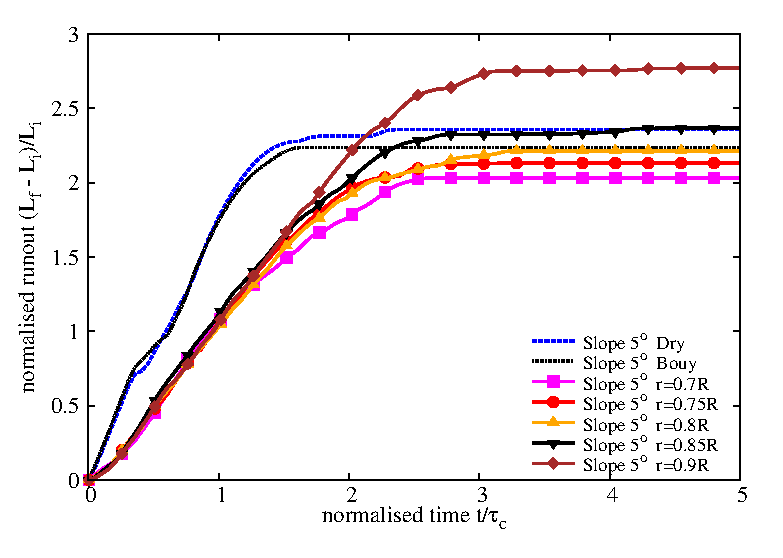
\includegraphics[width=0.97\columnwidth]{Runout_loose_5}
\caption{Evolution of run-out with time for different permeability (loose slope \SI{5}{\degree})}
\label{fig:run5}
\end{figure}


\begin{figure}
\centering
\includegraphics[width=0.97\columnwidth]{Height_loose_5}
\caption{Evolution of height with time for different permeability (loose slope \SI{5}{\degree})}
\label{fig:height5}
\end{figure}

\begin{figure}
\centering
\includegraphics[width=0.97\columnwidth]{KE_loose_5}
\caption{Evolution of Kinetic Energy with time for different permeability (loose slope \SI{5}{\degree})}
\label{fig:KE5}
\end{figure}

Positive pore-pressure generation at the base of the flow was observed for low permeable conditions. Inspection of the local packing density showed entrainment of water at the base of the flow, which can also be observed by the steep decrease in the packing density (see~\Cref{fig:voro5}) for the very low permeability condition (r = 0.9R). At the end of the flow ($t \ge 3 \times \tau_c$), the excess pore-pressure dissipates and the granular material, irrespective of their permeability, reaches almost the same packing density.

\begin{figure}
\centering
\includegraphics[width=0.97\columnwidth]{Voronoi_5}
\caption{Evolution of packing density with time for different permeability (loose slope \SI{5}{\degree})}
\label{fig:voro5}
\end{figure}

\subsection{SUMMARY}

Two-dimensional LB-DEM simulations were performed to understand the behaviour of submarine granular flows. Unlike dry granular collapse, the run-out behaviour in fluid is dictated by the initial volume fraction. Granular columns with loose packing tend to flow longer in comparison to dense columns, due to entrainment of water at the base resulting in lubrication. The loose column when it starts flowing expands and ejects liquid, leading to a partial fluidization of the material. However, with increase in the slope angle, the run-out in fluid is influenced by the viscous drag on the granular materials. The run-out distance in fluid increases with decrease in permeability. More research work is required to characterise the flow behaviour of granular materials, especially in submerged conditions.
